\documentclass{article}
\usepackage{graphicx}
\usepackage{hyperref}
\usepackage{caption}
\usepackage{subcaption}
\usepackage[dutch]{babel}

\begin{document}

\begin{center}
	\huge{Wiskunde in Kunst}\\
	\LARGE{Opdracht 1} \\
	
	\vspace{2cm}
	
	\Large{Circle Limit III}\\
	\large{\textit{M. C. Escher}}
	
	\begin{figure}[htp]
		\centering
		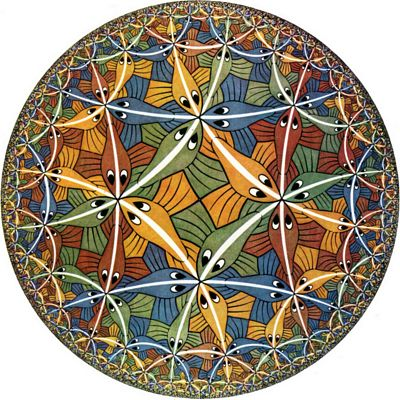
\includegraphics[scale=1.00]{Escher_Circle_Limit_III.jpg}
		\label{}
	\end{figure}
	
	\vfill
	\Large{Marcelo Dias Avelino} \hfill \large{0840416}
\end{center}

\pagebreak

\section{Kunstwerk}

De kunstwerk \textit{Circle Limit III} is een houtsnede stuk gemaakt door de nederlandse kunstenaar Maurits Cornelis Escher (meestal gerefereerd als M. C. Escher). Escher heeft dit kunstwerk gemaakt in 1959 in zijn huis in Baarn, Utrecht. Hij verhuisde hierheen in 1941 vanuit Brussel vanwege de tweede wereld oorlog. Hier heeft hij de grootste gedeelte van zijn meest bekende kunstwerken, zoals \textit{Drawing Hands}, \textit{Relativity} en \textit{Waterfall}, gemaakt.

\begin{figure}[h]
        \centering
        \begin{subfigure}{0.33\textwidth}
                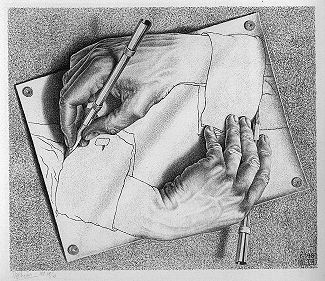
\includegraphics[width=\textwidth]{DrawingHands}
                \caption{\textit{Drawing Hands}}
        \end{subfigure}%
       	~ 
        \begin{subfigure}{0.33\textwidth}
                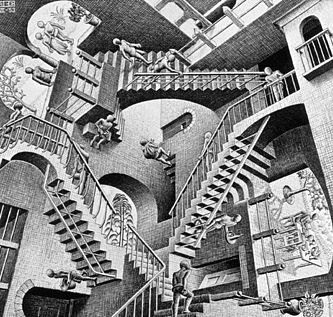
\includegraphics[width=\textwidth]{Escher's_Relativity}
                \caption{\textit{Relativity}}
        \end{subfigure}%
        ~ 
        \begin{subfigure}{0.33\textwidth}
                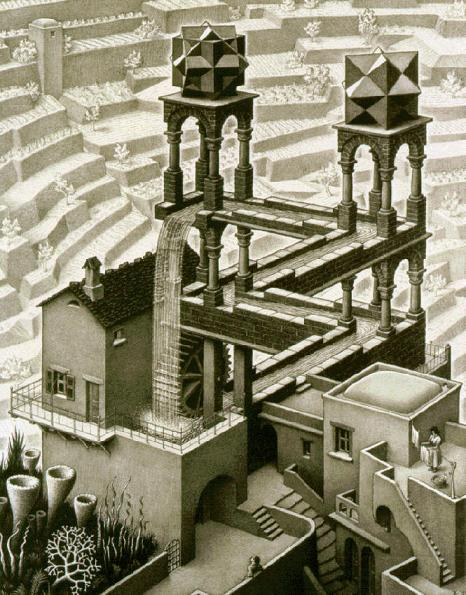
\includegraphics[width=\textwidth]{Escher_Waterfall}
                \caption{\textit{Waterfall}}
        \end{subfigure}%
        \caption{Drie bekende kunstwerken van Escher.}
        \label{fig:structCompare}
\end{figure}

\noindent Escher's inspiratie voor de \textit{Circle Limit III} kwam van een bezoek aan Alhambra. Alhambra is een paleis in Spanje waar zich muren bevinden die versierd zijn met repetitieve patronen die elkaar niet overlappen, zo genaamd tesselatie of betegeling. De naam tesselatie komt uit de latijn \textit{tessella}, dat staat voor kleine stuk klei, steen of glas die gebruikt wordt om moza\"iek te maken. Er zijn meerdere soorten tesselatie, maar het meeste gebruikte en diegene waar Escher zijn inspiratie vandaan heeft gehaald, samen met \textit{rotatiesymmetrisch} tesselatie waarbij de element alleen gedraaid wordt, zijn zogenaamde \textit{translatiesymmetrisch} betegeling. Dit zijn herhalende patronen waarbij de vorm van het element ongewijzigd blijft en alleen verschoven worden. In de wiskunde zijn deze patronen gecategoriseerd in zo genaamde behangpatroongroepen. Er zijn 17 verschillende patronen en deze zijn allemaal te vinden in Alhambra. 

De oudste gevonden werken van tesselatie zijn gevonden in de rijk van Sumer, waar de huidig Irak zich bevindt. Soemeri\"ers maakten al in 4500 voor Christus ook gebruik van in de vorm van kleitegels om muren te versieren.
\\ \\
Dit kunstwerk is verder ook gebaseerd op een afbeelding die zich bevond in een paper van meetkundiger Donald Coxeter genaamd \textit{``Crystal Symmetry and its Generalizations''}. De afbeelding, die te zien is in Figuur \ref{fig:hyperbolic-domains}, weergeeft een tesselatie met rechthoekig driehoeken met hoeken van 30, 45, and 90 graden binnen een hyperbolische vlakte.
Een hyperbolische vlakte is een vlakte waar twee parallel lopende lijnen steeds verder weg van elkaar buigen hoe verder je elke kant op gaat. Een andere voorbeeld van zo'n een vlakte is een zadel, zoals te zien is in Figuur \ref{fig:curved}. Er gelden niet dezelfde regels in een hyperbolische vlakte als in een vlakke twee dimensioneel vlakte, waardoor het mogelijk is om driehoeken te hebben met een optelling van hoeken over 180 graden. Het kunstwerk \textit{Circle Limit III} is sterk gebaseerd op de afbeelding uit Coxeter's paper.

\begin{figure}[Hh]
        \centering
        \begin{subfigure}{0.415\textwidth}
            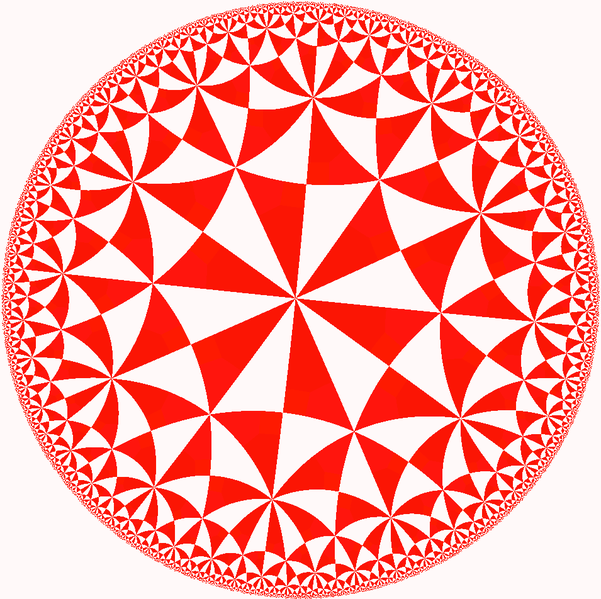
\includegraphics[width=\textwidth]{hyperbolic_domains}
            \caption{\textit{Afbeelding uit Coxeter's paper.}}
			\label{fig:hyperbolic-domains}
        \end{subfigure}%
       	~ 
        \begin{subfigure}{0.5\textwidth}
			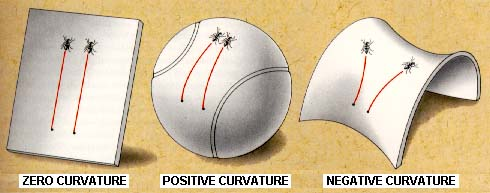
\includegraphics[width=\textwidth]{curved}
            \caption{\textit{Een zadel is een hyperbolische vlakte.}}
			\label{fig:curved}
        \end{subfigure}%
        \caption{Hyperbolische vlaktes}
        \label{fig:structCompare}
\end{figure}

Wanneer het bekend is wat de bronnen van inspiratie van M. C. Esther waren, is het makkelijker en duidelijker waar zijn kunsttukken uit opgebouwd zijn. 

\pagebreak

\begin{thebibliography}{9}

\bibitem{}
	\url{http://en.wikipedia.org/wiki/Circle_Limit_III}

\bibitem{}
	\url{http://nl.wikipedia.org/wiki/Hyperbolische_meetkunde}

\bibitem{}
	\url{http://en.wikipedia.org/wiki/Hyperbolic_geometry}

\bibitem{}
	\url{http://en.wikipedia.org/wiki/Wallpaper_group}

\bibitem{}
	\url{http://en.wikipedia.org/wiki/Tessellation}

\bibitem{}
	\url{http://nl.wikipedia.org/wiki/Betegeling}

\bibitem{}
	\url{http://nl.wikipedia.org/wiki/Houtsnede}

\bibitem{}
	\url{http://en.wikipedia.org/wiki/Non-Euclidean_geometry}

\bibitem{}
	\url{http://nl.wikipedia.org/wiki/Niet-euclidische_meetkunde}

\bibitem{}
	\url{http://nl.wikipedia.org/wiki/Maurits_Cornelis_Escher}

\bibitem{}
	\url{http://en.wikipedia.org/wiki/M._C._Escher}

\bibitem{}
	\url{http://en.wikipedia.org/wiki/Baarn}

\bibitem{}
	\url{http://nl.wikipedia.org/wiki/Donald_Coxeter}

	
\end{thebibliography}

\end{document}
